\documentclass[nobib]{tufte-handout}

\newcommand{\bra}[1]{\left(#1\right)}
\usepackage{amssymb}
\usepackage{hyperref}
\usepackage{pgfplots}
\usepackage[activate={true,nocompatibility},final,tracking=true,kerning=true,spacing=true,factor=1100,stretch=10,shrink=10]{microtype}
\usepackage{color}
\usepackage{steinmetz}
\usepackage{placeins}
\usepackage{marginfix}
\usepackage{array}
\usepackage{tikz}
\usepackage{amsmath,amsthm}
\usetikzlibrary{shapes, arrows, positioning, calc}
\tikzset{block/.style={draw, rectangle, minimum height=1.5em, minimum width=3em},
         sum/.style={draw, circle, inner sep=0pt, minimum size=2mm},
         >=latex'}
\usepackage{listings}
\usepackage{forest}
\usepackage{caption}
\DeclareCaptionFont{white}{\color{white}}
\DeclareCaptionFormat{listing}{\colorbox{gray}{\parbox{\textwidth}{#1#2#3}}}
\captionsetup[lstlisting]{format=listing,labelfont=white,textfont=white}
\usepackage{graphicx}
\setkeys{Gin}{width=\linewidth,totalheight=\textheight,keepaspectratio}
\graphicspath{{.}}

\title{ECE 30200 - Probabilistic Methods in Electrical and Computer Engineering}
\author{Zeke Ulrich}
\date{\today}  % if the \date{} command is left out, the current date will be used

\usepackage{booktabs}
\usepackage{units}
\usepackage{fancyvrb}
\fvset{fontsize=\normalsize}
\usepackage{multicol}

\begin{document}

\maketitle

\tableofcontents

\pagebreak

\section{Background}

The following formulas will be instrumental and may be familar.

\subsection{Series}
\begin{equation}
    \sum_{k=0}^{n} r^k = \frac{1 - r^{n + 1}}{1 - r}
\end{equation}
\begin{equation}
    \sum_{n=1}^{\infty} \frac{1}{n^2} = \frac{\pi^2}{6}
\end{equation}
\begin{equation}
    \sum_{k=1}^{\infty}kr^{k - 1} = \frac{1}{(1 - r)^2}
\end{equation}

\subsection{Combinatorics}
\begin{equation}
    {n\choose k} = \frac{n!}{k!(n - k)!}
\end{equation}
\begin{equation}
    (a + b)^n = \sum_{k=0}^{n} {n\choose k} a^{n - k}b^k
\end{equation}
\begin{equation}
    {n\choose k} + {n\choose k-1} = {n + 1\choose k}
\end{equation}
\begin{equation}
    P(n, k) = \frac{n!}{(n-k)!}
\end{equation}
where $P(n, k)$ is the number of ways to arrange $k$ objects out of $n$ (permutations).
\begin{equation}
    C(n, k) = {n\choose k} = \frac{n!}{k!(n-k)!}
\end{equation}
where $C(n, k)$ is the number of ways to choose $k$ objects out of $n$ (combinations).

\subsection{Approximations}
\begin{align}
    f(x) & = f(a) + f'(a)(x - a) + \frac{f''(a)}{2!}(x - a)^2 + \dots \\
         & = \sum_{n=0}^{\infty} \frac{f^{(n)}(a)}{n!}(x - a)^n
\end{align}
\begin{align}
    1 + x + \frac{x^2}{2!} + \frac{x^3}{3!} + \dots & = \sum_{k=0}^{\infty} \frac{x^k}{k!} \\
                                                    & = e^x
\end{align}
\begin{align}
    \sin(x) & = x - \frac{x^3}{3!} + \frac{x^5}{5!} - \frac{x^7}{7!} + \dots \\
            & = \sum_{n=0}^{\infty} (-1)^n \frac{x^{2n+1}}{(2n+1)!}
\end{align}
\begin{align}
    \cos(x) & = 1 - \frac{x^2}{2!} + \frac{x^4}{4!} - \frac{x^6}{6!} + \dots \\
            & = \sum_{n=0}^{\infty} (-1)^n \frac{x^{2n}}{(2n)!}
\end{align}
\begin{align}
    \ln(1 + x) & = x - \frac{x^2}{2} + \frac{x^3}{3} - \frac{x^4}{4} + \dots \\
               & = \sum_{n=1}^{\infty} (-1)^{n+1} \frac{x^n}{n}
\end{align}

\subsection{Calculus}
\begin{equation}
    \frac{d}{dx} \int_{a}^{x} f(t)\,dt = f(x)
\end{equation}
\begin{equation}
    \int_{a}^{b} f'(x)\,dx = f(b) - f(a)
\end{equation}
\begin{equation}
    \int f(g(x))g'(x)\,dx = \int f(u)\,du
\end{equation}
\begin{equation}
    \int u\,dv = uv - \int v\,du
\end{equation}
\begin{equation}
    \int \frac{1}{(x-a)(x-b)}\,dx = \frac{1}{b-a} \ln\left|\frac{x-a}{x-b}\right| + C
\end{equation}

\subsection{Linear Algebra}
\begin{equation}
    \vec{y} = \beta_1 \vec{x_1} + \beta_2 \vec{x_2} + \cdots + \beta_N \vec{x_N}
\end{equation}
\begin{align}
    \langle \vec{a}, \vec{b} \rangle & = \vec{a}\vec{b}^{T}     \\
                                     & = \sum_{i=1}^{n} a_i b_i
\end{align}
where $\langle \vec{a}, \vec{b} \rangle$ denotes the inner product of vectors $\vec{a}$ and $\vec{b}$.
\begin{equation}
    \|\vec{x}\|_p = \left( \sum_{i=1}^{n} |x_i|^p \right)^{1/p}
\end{equation}
where $\|\vec{x}\|_p$ is the $p$-norm (or $\ell_p$-norm) of vector $\vec{x}$.
\begin{equation}
    \cos(\theta) = \frac{\langle \vec{a}, \vec{b} \rangle}{\|\vec{a}\|_2 \|\vec{b}\|_2}
\end{equation}
where $\theta$ is the angle between vectors $\vec{a}$ and $\vec{b}$.
\begin{equation}
    \hat{\beta} = (\mathbf{X}^T \mathbf{X})^{-1} \mathbf{X}^T \vec{y}
\end{equation}
where $\hat{\beta}$ is the vector of least squares coefficients, $\mathbf{X}$ is the data matrix, and $\vec{y}$ is the target vector

\subsection{Set Theory}
Some important properties of set operations are:
\begin{itemize}
    \item \textbf{Commutativity:}
          \begin{align}
              A \cup B & = B \cup A \\
              A \cap B & = B \cap A
          \end{align}
    \item \textbf{Associativity:}
          \begin{align}
              (A \cup B) \cup C & = A \cup (B \cup C) \\
              (A \cap B) \cap C & = A \cap (B \cap C)
          \end{align}
    \item \textbf{Distributivity:}
          \begin{align}
              A \cup (B \cap C) & = (A \cup B) \cap (A \cup C) \\
              A \cap (B \cup C) & = (A \cap B) \cup (A \cap C)
          \end{align}
    \item \textbf{Identity:}
          \begin{align}
              A \cup \emptyset & = A \\
              A \cap \Omega    & = A
          \end{align}
    \item \textbf{Complement:}
          \begin{align}
              A \cup A^c & = \Omega    \\
              A \cap A^c & = \emptyset
          \end{align}
\end{itemize}

\subsection{Probability Laws}
A probability law must satisfy three axioms:
\begin{enumerate}
    \item Non-negativity: $P(A) \geq 0 \forall A \in F$
    \item Normalization: $P(\Omega) = 1$
    \item Additivity: For any disjoint subsets $\{A_1, A_2, \dots\}$,
          it holds that
          \[P\left[\bigcup_{n=1}^{\infty}A_n\right] = \sum_{n=1}^{\infty}P\left[A_n\right]\]
\end{enumerate}

\subsection{Probability Properties}
\begin{equation}
    P\left[A \cup B\right] = P\left[A\right] + P\left[B\right] - P\left[A \cap B\right]
\end{equation}
\begin{equation}
    P\left[A \cup B\right] \leq P\left[A\right] + P\left[B\right]
\end{equation}
\begin{equation}
    A \subseteq B \implies P\left[A\right] \leq P\left[B\right]
\end{equation}
\section{Formal Definitions}

\subsection{Outcomes}
An \emph{outcome} is the result of some \emph{experiment}.
If that experiment is flipping a coin, the outcome is either
heads or tails. We could express the outcome of heads as $H$,
and the outcome of tails as $T$. The set of all possible
outcomes for an experiment is known as a sample space and is
denoted by $\Omega$. In this case $\Omega = \{H, T\}$.

\subsection{Events}
An \emph{event} $F$ is a subset of the sample space $\Omega$.
The formal definitions of probability are expressed with set
notation. So the event where we have neither heads nor tails is
written as $\{\}$. The event of heads could be expressed as
$\{H\}$, and the event of tails could be expressed as $\{T\}$.
The event of either heads or tails is $\{H, T\}$.

\subsection{Probability Laws}
A \emph{probability law} is a function $P$ that maps an event $A$
to a real number in $[0, 1]$. For the coin example, the probability
law might be $P(\{\}) = 0$, $P(\{H\}) = 0.5$, $P(\{T\}) = 0.5$, and
$P(\{\Omega\}) = 1$. A probability law must satisfy three axioms:
\begin{enumerate}
    \item Non-negativity: $P(A) \geq 0 \forall A \in F$
    \item Normalization: $P(\Omega) = 1$
    \item Additivity: For any disjoint subsets $\{A_1, A_2, \dots\}$,
          it holds that
          \[P\left[\bigcup_{n=1}^{\infty}A_n\right] = \sum_{n=1}^{\infty}P\left[A_n\right]\]
\end{enumerate}

\subsection{Probability Space}
A probability space is a triplet $\Omega, F, P$.

\subsection{Probability Properties}
\begin{equation}
    P\left[A \cup B\right] = P\left[A\right] + P\left[B\right] - P\left[A \cap B\right]
\end{equation}
\begin{equation}
    P\left[A \cup B\right] \leq P\left[A\right] + P\left[B\right]
\end{equation}
\begin{equation}
    A \subseteq B \implies P\left[A\right] \leq P\left[B\right]
\end{equation}
\begin{equation}
    P\left[A | B\right] = \frac{P[A \cap B]}{P[B]}
\end{equation}

Outcomes are statistically \emph{independent} if
$P(A|B) = P(A)$ (assuming P(B) > 0), or
equivalently $P(A \cap B) = P(A)P(B)$.

A \emph{random variable} $X$ is a function $X : \Omega \implies \Re$
that maps an outcome $\epsilon \in \Omega$ to a number $X(\epsilon)$ on the real line.
We call it a variable because it has multiple states. The mapping $X$

\emph{Bayes Theorem} states that for any two events $A$ and $B$ such that $P[A] > 0$ and
$P[B] > 0$,
\begin{equation}
    P[A|B] = \frac{P[B|A]P[A]}{P[B]}
\end{equation}

The \emph{Law of Total Probability} states that if
$\{A_1, A_2, \dots, A_n\}$ is a partition of $\Omega$,
then for any $B \subseteq \Omega$,
\begin{equation}
    P[B] = \sum_{i = 1}^{n} P[B|A_i]P[A_i]
\end{equation}
\section{PMFs and CDFs}

The \emph{probability mass function} (PMF) $p_X(a)$
of a random variable $X$ specifies the probability of
obtaining a number $X(\epsilon) = a$. We denote a PMF as
\begin{equation}
    p_X(a) = P[X = a]
\end{equation}
PMFs are represented with histograms.
\begin{figure}[h]
    \centering
    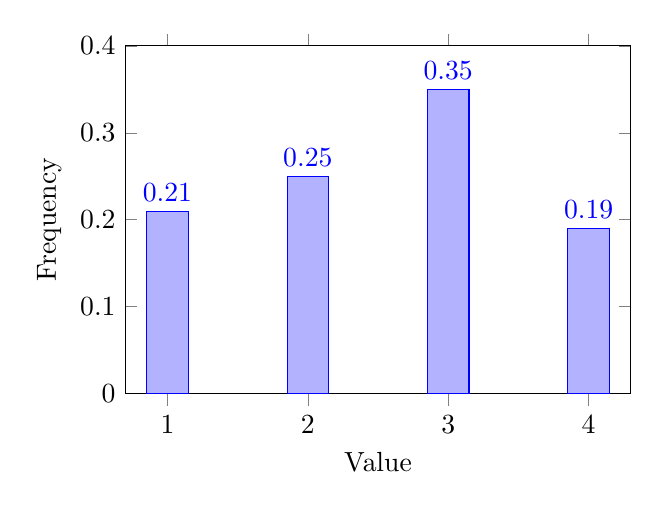
\begin{tikzpicture}
        \begin{axis}[
                ybar,
                bar width=15pt,
                xlabel={Value},
                ylabel={Frequency},
                xtick=data,
                ymin=0,
                ymax=0.4,
                nodes near coords,
                width=8cm,
                height=6cm
            ]
            \addplot coordinates {(1,0.21) (2,0.25) (3,0.35) (4,0.19)};
        \end{axis}
    \end{tikzpicture}
    \caption{PMF}
\end{figure}
A PMF should satisfy
\begin{equation}
    \sum_{x\in X(\Omega)} p_X(x) = 1
\end{equation}

The \emph{cumulative distribution function} is given by
\begin{align}
    F_X(x) & = P\left[X \leq x\right] \\
           & = \sum_{u \leq x} p_X(u)
\end{align}
and represents the sum of every impulse
of the PMF up to $x$.

\appendix

\section{Reference}
\setcounter{equation}{0}


\subsection{Series}
\begin{equation}
    \sum_{k=0}^{n} r^k = \frac{1 - r^{n + 1}}{1 - r}
\end{equation}
\begin{equation}
    \sum_{n=1}^{\infty} \frac{1}{n^2} = \frac{\pi^2}{6}
\end{equation}
\begin{equation}
    \sum_{k=1}^{\infty}kr^{k - 1} = \frac{1}{(1 - r)^2}
\end{equation}

\subsection{Combinatorics}
\begin{equation}
    {n\choose k} = \frac{n!}{k!(n - k)!}
\end{equation}
\begin{equation}
    (a + b)^n = \sum_{k=0}^{n} {n\choose k} a^{n - k}b^k
\end{equation}
\begin{equation}
    {n\choose k} + {n\choose k-1} = {n + 1\choose k}
\end{equation}
\begin{equation}
    P(n, k) = \frac{n!}{(n-k)!}
\end{equation}
where $P(n, k)$ is the number of ways to arrange $k$ objects out of $n$ (permutations).
\begin{equation}
    C(n, k) = {n\choose k} = \frac{n!}{k!(n-k)!}
\end{equation}
where $C(n, k)$ is the number of ways to choose $k$ objects out of $n$ (combinations).

\subsection{Approximations}
\begin{align}
    f(x) & = f(a) + f'(a)(x - a) + \frac{f''(a)}{2!}(x - a)^2 + \dots \\
         & = \sum_{n=0}^{\infty} \frac{f^{(n)}(a)}{n!}(x - a)^n
\end{align}
\begin{align}
    1 + x + \frac{x^2}{2!} + \frac{x^3}{3!} + \dots & = \sum_{k=0}^{\infty} \frac{x^k}{k!} \\
                                                    & = e^x
\end{align}
\begin{align}
    \sin(x) & = x - \frac{x^3}{3!} + \frac{x^5}{5!} - \frac{x^7}{7!} + \dots \\
            & = \sum_{n=0}^{\infty} (-1)^n \frac{x^{2n+1}}{(2n+1)!}
\end{align}
\begin{align}
    \cos(x) & = 1 - \frac{x^2}{2!} + \frac{x^4}{4!} - \frac{x^6}{6!} + \dots \\
            & = \sum_{n=0}^{\infty} (-1)^n \frac{x^{2n}}{(2n)!}
\end{align}
\begin{align}
    \ln(1 + x) & = x - \frac{x^2}{2} + \frac{x^3}{3} - \frac{x^4}{4} + \dots \\
               & = \sum_{n=1}^{\infty} (-1)^{n+1} \frac{x^n}{n}
\end{align}

\subsection{Calculus}
\begin{equation}
    \frac{d}{dx} \int_{a}^{x} f(t)\,dt = f(x)
\end{equation}
\begin{equation}
    \int_{a}^{b} f'(x)\,dx = f(b) - f(a)
\end{equation}
\begin{equation}
    \int f(g(x))g'(x)\,dx = \int f(u)\,du
\end{equation}
\begin{equation}
    \int u\,dv = uv - \int v\,du
\end{equation}
\begin{equation}
    \int \frac{1}{(x-a)(x-b)}\,dx = \frac{1}{b-a} \ln\left|\frac{x-a}{x-b}\right| + C
\end{equation}

\subsection{Linear Algebra}
\begin{equation}
    \vec{y} = \beta_1 \vec{x_1} + \beta_2 \vec{x_2} + \cdots + \beta_N \vec{x_N}
\end{equation}
\begin{align}
    \langle \vec{a}, \vec{b} \rangle & = \vec{a}\vec{b}^{T}     \\
                                     & = \sum_{i=1}^{n} a_i b_i
\end{align}
where $\langle \vec{a}, \vec{b} \rangle$ denotes the inner product of vectors $\vec{a}$ and $\vec{b}$.
\begin{equation}
    \|\vec{x}\|_p = \left( \sum_{i=1}^{n} |x_i|^p \right)^{1/p}
\end{equation}
where $\|\vec{x}\|_p$ is the $p$-norm (or $\ell_p$-norm) of vector $\vec{x}$.
\begin{equation}
    \cos(\theta) = \frac{\langle \vec{a}, \vec{b} \rangle}{\|\vec{a}\|_2 \|\vec{b}\|_2}
\end{equation}
where $\theta$ is the angle between vectors $\vec{a}$ and $\vec{b}$.
\begin{equation}
    \hat{\beta} = (\mathbf{X}^T \mathbf{X})^{-1} \mathbf{X}^T \vec{y}
\end{equation}
where $\hat{\beta}$ is the vector of least squares coefficients, $\mathbf{X}$ is the data matrix, and $\vec{y}$ is the target vector

\end{document}